\documentclass[a4paper,12pt]{article}
\usepackage[top = 2.5cm, bottom = 2.5cm, left = 2.5cm, right = 2.5cm]{geometry}
\usepackage[T1]{fontenc}
\usepackage[utf8]{inputenc}
\usepackage{multirow} 
\usepackage{booktabs} 
\usepackage{graphicx}
\usepackage[spanish]{babel}
\usepackage{setspace}
\setlength{\parindent}{0in}
\usepackage{float}
\usepackage{fancyhdr}
\usepackage{amsmath}
\usepackage{amssymb}
\usepackage{amsthm}
\usepackage[numbers]{natbib}
\newcommand\Mycite[1]{%
	\citeauthor{#1}~[\citeyear{#1}]}
\usepackage{graphicx}
\usepackage{subcaption}
\usepackage{booktabs}
\usepackage{etoolbox}
\usepackage{minibox}
\usepackage{hyperref}
\usepackage{xcolor}
\usepackage[skins]{tcolorbox}
%---------------------------

\newtcolorbox{cajita}[1][]{
	 #1
}

\newenvironment{sol}
{\renewcommand\qedsymbol{$\square$}\begin{proof}[\textbf{Solución.}]}
	{\end{proof}}

\newenvironment{dem}
{\renewcommand\qedsymbol{$\blacksquare$}\begin{proof}[\textbf{Demostración.}]}
	{\end{proof}}

\newtheorem{problema}{Problema}
\newtheorem{definicion}{Definición}
\newtheorem{ejemplo}{Ejemplo}
\newtheorem{teorema}{Teorema}
\newtheorem{corolario}{Corolario}[teorema]
\newtheorem{lema}[teorema]{Lema}
\newtheorem{prop}{Proposición}
\newtheorem*{nota}{\textbf{NOTA}}
\renewcommand\qedsymbol{$\blacksquare$}
\usepackage{svg}
\usepackage{tikz}
\usepackage[framemethod=default]{mdframed}
\global\mdfdefinestyle{exampledefault}{%
linecolor=lightgray,linewidth=1pt,%
leftmargin=1cm,rightmargin=1cm,
}




\newenvironment{noter}[1]{%
\mdfsetup{%
frametitle={\tikz\node[fill=white,rectangle,inner sep=0pt,outer sep=0pt]{#1};},
frametitleaboveskip=-0.5\ht\strutbox,
frametitlealignment=\raggedright
}%
\begin{mdframed}[style=exampledefault]
}{\end{mdframed}}
\newcommand{\linea}{\noindent\rule{\textwidth}{3pt}}
\newcommand{\linita}{\noindent\rule{\textwidth}{1pt}}

\AtBeginEnvironment{align}{\setcounter{equation}{0}}
\pagestyle{fancy}

\fancyhf{}









%----------------------------------------------------------
\lhead{\footnotesize Modelación y Simulación}
\rhead{\footnotesize  Rudik Roberto Rompich}
\cfoot{\footnotesize \thepage}


%--------------------------

\begin{document}
 \thispagestyle{empty} 
    \begin{tabular}{p{15.5cm}}
    \begin{tabbing}
    \textbf{Universidad del Valle de Guatemala} \\
    Departamento de Matemática\\
    Licenciatura en Matemática Aplicada\\\\
   \textbf{Estudiante:} Rudik Roberto Rompich\\
   \textbf{Correo:}  \href{mailto:rom19857@uvg.edu.gt}{rom19857@uvg.edu.gt}\\
   \textbf{Carné:} 19857
    \end{tabbing}
    \begin{center}
        CC3039 - Modelación y Simulación - Catedrático: Oseas Paredes\\
        \today
    \end{center}\\
    \hline
    \\
    \end{tabular} 
    \vspace*{0.3cm} 
    \begin{center} 
    {\Large \bf Microproyecto 1
} 
        \vspace{2mm}
    \end{center}
    \vspace{0.4cm}
%--------------------------

\begin{problema}
	Trosper Tire Company decidió contratar a un nuevo mecánico para que se encargue de todos los cambios para clientes que piden un nuevo juego de llantas. Dos mecánicos solicitaron el trabajo. Uno tiene experiencia limitada y puede ser contratado a \$14 por hora y puede atender a un promedio de tres clientes por hora. El otro tiene varios años de experiencia y puede atender a un promedio de cuatro clientes por hora, pero debe ser contratado a \$20 por hora. Suponga que los clientes llegan a Trosper a razón de dos por hora.
	\begin{enumerate}
		\item ¿Cuáles son las características de operación con cada mecánico, suponiendo llegadas Poisson y tiempos de servicio exponenciales?
		\begin{sol}
			A continuación se listan las características de operación de cada mecánico: 
			\begin{figure}[H]
				\centering
				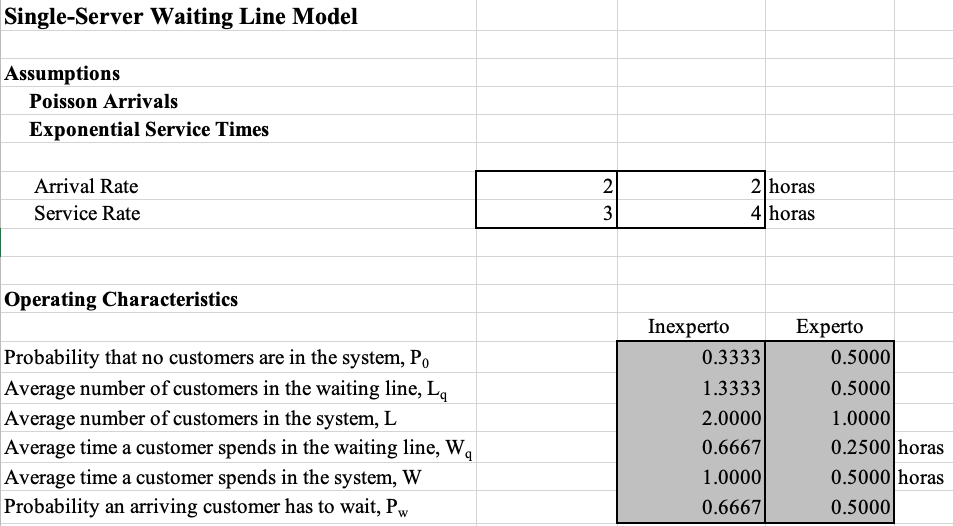
\includegraphics[scale=0.4]{Images/1}
				\caption{Plantilla de Quantitative Methods for Business de Andersen et al. }
			\end{figure}
		\end{sol}
		\item Si la empresa asigna un costo de \$30 por hora a un cliente que espera, ¿cuál mecánico ofrece el menor costo de operación?
		\begin{sol}
			El costo de operación se calcula así: 
			$$ \text{Operación}=\text{Costo\_espera}*\text{Promedio\_clientes\_en\_el\_sistema}+\text{Costo\_contratación} $$
			De los cuales obtenemos lo siguiente: 
			\begin{figure}[H]
				\centering
				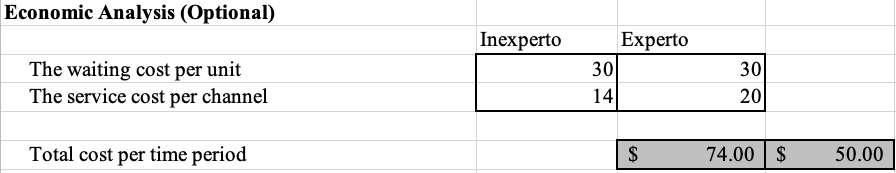
\includegraphics[scale=0.4]{Images/2}
				\caption{Plantilla de Quantitative Methods for Business de Andersen et al. }
			\end{figure}
		Por lo tanto, el mecánico experimentado tiene un menor costo de operación.
		\end{sol}
	\end{enumerate}
\end{problema}

\begin{problema}
	Agan Interior Design ofrece asesoría de decoración de casas y oficinas a sus clientes. En operación normal, llega un promedio de 2.5 clientes cada hora. Un asesor de diseño está disponible para responder las preguntas de los clientes y para recomendar productos. El asesor promedia 10 minutos con cada cliente.
	\begin{enumerate}
		\item Calcule las características de operación de la línea de espera de clientes, suponiendo llegadas Poisson y tiempos de servicio exponenciales.
		\begin{sol}
			Nótese que el servicio se trabajará en horas, por lo tanto son 6 clientes que se atienden por hora tal que: 
				\begin{figure}[H]
				\centering
				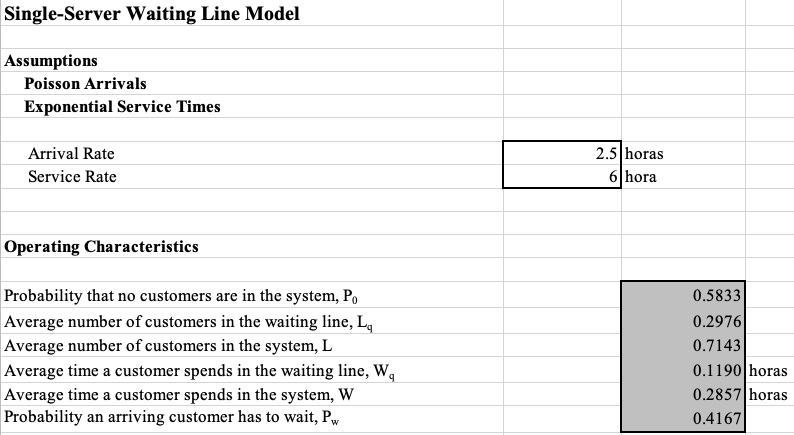
\includegraphics[scale=0.4]{Images/3}
				\caption{Plantilla de Quantitative Methods for Business de Andersen et al. }
			\end{figure}
		\end{sol}
		\item Las metas de servicio dictan que un cliente que llega no deberá esperar a que lo atiendan más de un promedio de 5 minutos. ¿Se está cumpliendo esta meta? Si no, ¿qué acción recomienda?
		\begin{sol}
			Tenemos en promedio de espera: 
			$$0.1190 \text{ hora}*\frac{60 \text{ minutos}}{1 \text{ hora}}= 7.14 \text{ minutos}. $$
			Por lo tanto, no se está cumpliendo la meta. Se recomienda que el asesor mejore sus tiempos de servicio o en su defecto, contratar a otro asesor. 
		\end{sol}
		\item Si el asesor puede reducir el tiempo empleado por cliente a 8 minutos, ¿cuál es la tasa media de servicios? ¿Se cumplirá con la meta de servicio?
		\begin{sol}
			Como los clientes son en horas, entonces \textbf{la tasa media de servicios} es 60/8=7.5 clientes por hora tal que, 
			\begin{figure}[H]
				\centering
				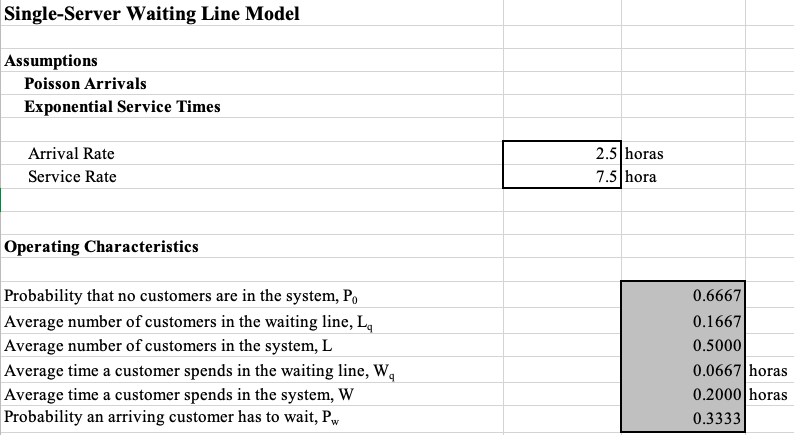
\includegraphics[scale=0.4]{Images/4}
				\caption{Plantilla de Quantitative Methods for Business de Andersen et al. }
			\end{figure}
		Por lo que 
				$$0.0667\text{ hora}*\frac{60 \text{ minutos}}{1 \text{ hora}}= 4.002 \text{ minutos}. $$
		\end{sol}
	Por lo tanto, con una tasa media de servicios de 7.5 clientes por hora, la meta sí se cumple. 
	\end{enumerate}
	
\end{problema}


\begin{problema}
	Todos los pasajeros en el aeropuerto regional de Lake City deben pasar por un área de revisión de seguridad antes de proseguir al área de abordaje. El aeropuerto cuenta con tres estaciones de revisión disponibles, y el director debe decidir cuántas tienen que estar abiertas en cualquier momento particular. La tasa de servicios para procesar los pasajeros en cada estación de revisión es de 3 pasajeros por minuto. En la mañana del lunes la tasa de llegadas es de 5.4 pasajeros por minuto. Suponga que los tiempos de procesamiento en esta estación de revisión siguen una distribución exponencial y que las llegadas siguen una distribución de Poisson.
	\begin{enumerate}
		\item Suponga que dos de las tres estaciones de revisión están abiertas en la mañana de los lunes. Calcule las características de operación de la estación de revisión.
		\begin{sol}
			Las características de operación son las siguientes: 
			\begin{figure}[H]
				\centering
				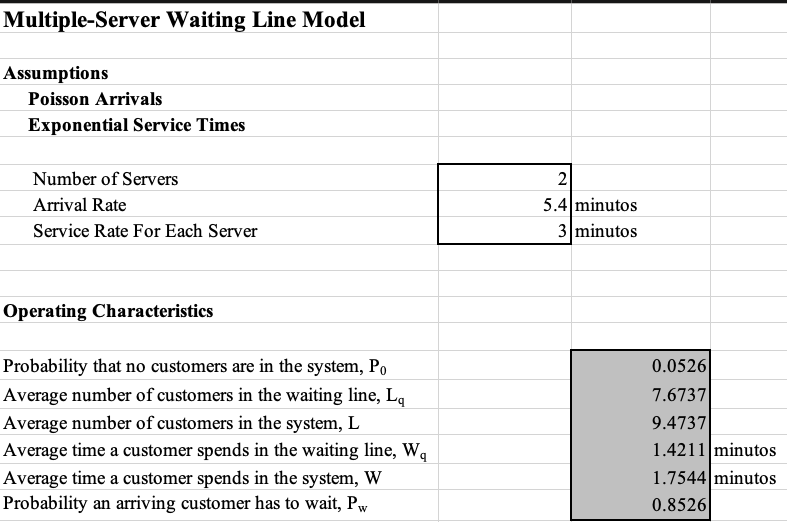
\includegraphics[scale=0.4]{Images/5}
				\caption{Plantilla de Quantitative Methods for Business de Andersen et al. }
			\end{figure}
		\end{sol}
		\item Debido a consideraciones de espacio, la meta del director de la estación es limitar el número de pasajeros promedio que esperan en línea a 10 o menos. ¿Serán capaces las dos estaciones de revisión de satisfacer la meta del director?
		\begin{sol}
			Sí, la meta del director se cumplirá; ya que en promedio solo 7.67 personas estarán en la línea de espera. 
		\end{sol}
		\item ¿Cuál es el tiempo promedio requerido para que un pasajero pase por la revisión de seguridad?
		\begin{sol}
			Es de aproximadamente 1.7544 minutos. 
		\end{sol}
	\end{enumerate}
\end{problema}


\begin{problema}
	Remítase a la situación de Agan Interior Design en el problema 2. A la gerencia de Agan le gustaría evaluar dos alternativas:
	\begin{enumerate}
		\item Utilizar un asesor con un tiempo de servicio promedio de 8 minutos por cliente.
		\begin{figure}[H]
			\centering
			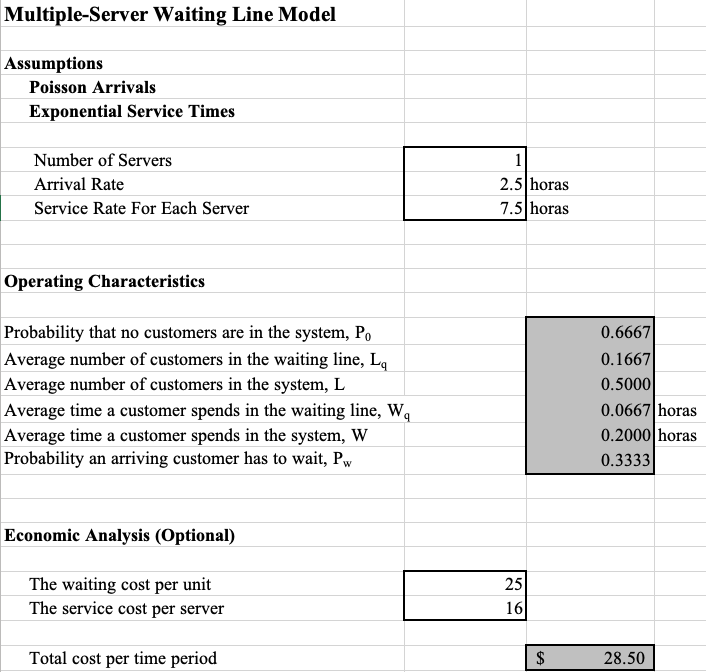
\includegraphics[scale=0.4]{Images/6}
			\caption{Plantilla de Quantitative Methods for Business de Andersen et al. }
		\end{figure}
		\item Utilizar dos asesores, cada uno con tiempo de servicio promedio de 10 minutos por cliente.
		\begin{figure}[H]
			\centering
			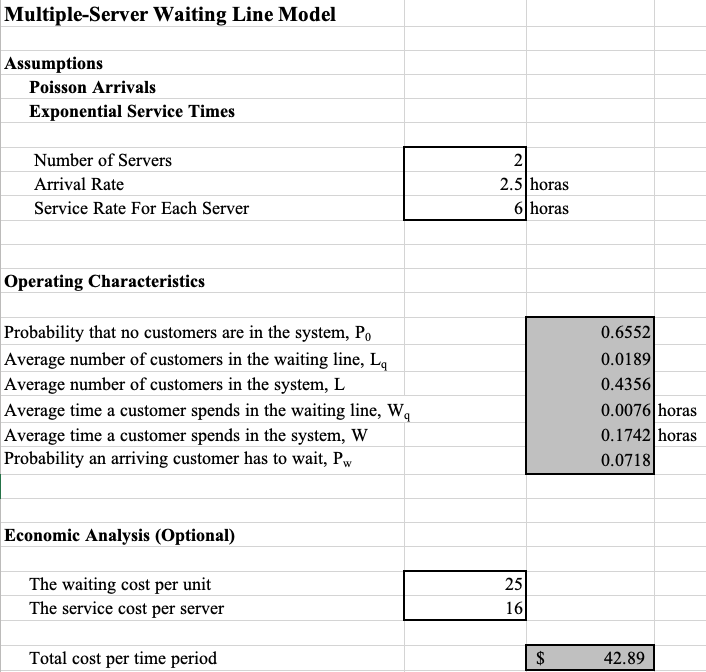
\includegraphics[scale=0.4]{Images/7}
			\caption{Plantilla de Quantitative Methods for Business de Andersen et al. }
		\end{figure}
	\end{enumerate}
	
	Si el salario de los asesores es de \$16 por hora y el costo del tiempo de espera de cada cliente es de \$25 por hora antes de ser atendido, ¿Deberá Agan ampliar el sistema a dos asesores? Explique.
	\begin{sol}
		El resultado dependerá de los objetivos específicos de la empresa, sin embargo nótese que con un asesor y 8 minutos por servicio el costo es de \$ 28.50 mientras que con dos asesores y 10 minutos por servicio el costo es de \$42.89. Por lo que la opción de un asesor parece ser la mejor y no sería necesario ampliar a 2 asesores. 
	\end{sol}
	
\end{problema}

\begin{problema}
	Cinco asistentes administrativos utilizan una copiadora. El tiempo promedio entre llegadas de cada asistente es de 40 minutos, el cual equivale a una tasa de llegadas de $1/40$=0.025 llegadas por minuto. El tiempo medio que un asistente pasa en la copiadora es de 5 minutos, el cual equivale a una tasa de servicios de 1/5=0.20 por minuto. Utilice el modelo M/M/1 con una población finita para determinar lo siguiente:
	\begin{figure}[H]
		\centering
		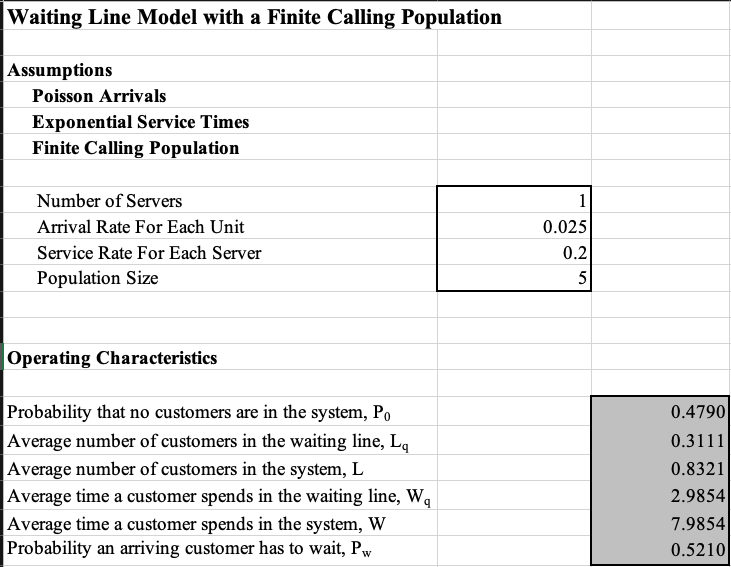
\includegraphics[scale=0.4]{Images/8}
		\caption{Plantilla de Quantitative Methods for Business de Andersen et al. }
	\end{figure}
	\begin{enumerate}
		\item La probabilidad de que la copiadora esté desocupada.
		\begin{sol}
			$P_0=0.4790$. 
		\end{sol}
		\item El número promedio de asistentes administrativos en la línea de espera.
		\begin{sol}
			$L_q=0.3110$ asistentes.
		\end{sol}
		\item El número promedio de asistentes administrativos en la copiadora.
		\begin{sol}
			$L=0.8321$ asistentes. 
		\end{sol}
		\item El tiempo promedio que un asistente pasa en espera de la copiadora.
		\begin{sol}
			$W_q=2.9854$ minutos. 
		\end{sol}
		\item El tiempo promedio que un asistente pasa en la copiadora.
		\begin{sol}
			$W=7.9854$ minutos.
		\end{sol}
		\item Durante un día de trabajo de 8 horas.
		\begin{enumerate}
			\item ¿Cuántos minutos pasa un asistente en la copiadora? 
			\begin{sol}
				Procederemos a calcular la cantidad de veces que se va a la fotocopiadora, tal que: 
				$$8 \text{ horas} * \frac{60 \text{ minutos} }{1 \text{ hora} }* 0.025=12 \text{ viajes al día.}$$
				Entonces, los minutos que pasa un asistente en la fotocopiadora es: 
				$$12 \text{ viajes} * 7.9854\text{ minutos}= 95.8 \text{ minutos por día.}$$
			\end{sol}
			\item ¿Cuánto de este tiempo es de espera?
			\begin{sol}
				El tiempo de espera es: 
				$$12 \text{ viajes} * 2.9854\text{ minutos}= 35.8 \text{ minutos por día.}$$
			\end{sol}
		\end{enumerate}
		
		\item ¿La gerencia deberá considerar adquirir una segunda copiadora? Explique.
		\begin{sol}
			Para responder la pregunta, vamos a calcular el tiempo que se pierde por esperar a utilizar la copiadora, tal que 
			$$35.8 \text{ minutos por día.}*5 \text { asistentes} =175 \text{ minutos} = 3 \text{ horas}.$$
			Por lo tanto, 3 horas de productividad son las que se pierden únicamente esperando; por lo que se podría concluir que sí sería necesario adquirir otra copiadora. 
		\end{sol}
	\end{enumerate}
	
	
\end{problema}

%---------------------------
%\bibliographystyle{apa}
%\bibliography{referencias.bib}

\end{document}